% =============================================================================
%  SCHEMA « LE MAILLON MANQUANT », diapositive du probleme (soutenance ENSAE)
%
%  Taille finale : 11,4 x 3,6 pouces, pose tel quel sur la diapositive.
%  Voie du haut : ce que DORA rend observable, jusqu'au besoin de capital ; le lien
%  entre l'etat de conformite et la chaine des pertes manque (accent rouge).
%  Voie du bas : la Formule Standard, qui ne recoit rien de l'etat de conformite.
%
%  AIDE A LA LECTURE (consigne de Hugo Rapior du 22 octobre) : deux fonds separent
%  l'ACTUEL (gris : ce qui existe aujourd'hui, DORA observable et Formule Standard)
%  du FUTUR (bleu a liseré rouge : ce que le memoire propose de construire, la chaine
%  incidents, charge annuelle, besoin de capital reliee a l'etat de conformite).
%  La legende en bas donne la cle de lecture. Aucun nombre, aucune formule ajoutes.
%
%  Libelles repris du rapport (main_ensae.pdf), sources dans chapitres_sfe/ :
%    rend observable, aucun dispositif prudentiel ... en capital : 00_introduction.tex l. 25-26
%    forfait, primes ou provisions techniques, meme bilan, meme charge, maturite sur
%      les cinq piliers : 00_introduction.tex l. 26-29
%    charge annuelle de pertes, quantile a 99,5 %, besoin de capital : 00_introduction.tex l. 43-45
%    P1 a P5 et leurs intitules : tableau des notations, annexe_b_parametres_notations.tex l. 132
%    etat de conformite par pilier : 03_donnees.tex l. 290
%    incidents TIC : 03_donnees.tex l. 127 ; propagation entre piliers : 04_frequence_severite.tex l. 118
%    plat en conformite : 01_contexte.tex l. 305
%
%  Les blocs n'ont pas de largeur imposee : chaque ligne est coupee a la main par \\,
%  si bien qu'aucune cesure ne peut couper un mot.
% =============================================================================
\documentclass[tikz,border=6pt]{standalone}
% =============================================================================
%  PREAMBULE COMMUN DES SCHEMAS DU SUPPORT DE SOUTENANCE (ENSAE, octobre 2026)
%
%  Les schemas sont des VISUELS DE DIAPOSITIVE, pas des figures de donnees : ils
%  prennent donc la palette du gabarit de presentation Nexialog, recopiee de
%  build_soutenance_ppt.py, et jamais celle de style_nexialog.py, qui reste la
%  source unique des couleurs des figures du memoire.
%
%  AUCUN NOMBRE DE RESULTAT N'Y FIGURE. Un nombre dessine dans une image echappe
%  au controle du support, qui verifie chaque nombre de texte contre le rapport.
%  Les schemas portent des symboles et des equations, recopiees du rapport.
%
%  Polices : Segoe UI pour le texte, comme le corps du gabarit ; Latin Modern Math
%  pour les formules, celle du rapport. Chaque schema se dessine A SA TAILLE FINALE
%  sur la diapositive, si bien qu'un corps de 14 pt ici vaut 14 pt a l'ecran.
% =============================================================================
\usepackage{fontspec}
\usepackage{unicode-math}
\setmainfont{Segoe UI}
\setsansfont{Segoe UI}
\setmathfont{latinmodern-math.otf}
\usetikzlibrary{positioning,arrows.meta,calc,fit,backgrounds,shapes.geometric,decorations.pathreplacing}

\definecolor{ardoise}{HTML}{223E55}   % titres et aplats du gabarit
\definecolor{profond}{HTML}{192E3F}
\definecolor{acier}{HTML}{435B6E}
\definecolor{encre}{HTML}{122738}     % texte courant
\definecolor{gris}{HTML}{595959}      % texte secondaire
\definecolor{accent}{HTML}{B10031}    % rouge de marque
\definecolor{clair}{HTML}{F2F2F2}
\definecolor{filet}{HTML}{D9D9D9}

\newcommand{\corps}{\fontsize{14}{17}\selectfont}
\newcommand{\petit}{\fontsize{12}{14.5}\selectfont}
\newcommand{\grand}{\fontsize{16}{19}\selectfont}
\tikzset{
  >={Stealth[length=7pt,width=6pt]},
  bloc/.style={draw=ardoise, line width=0.9pt, fill=white, rounded corners=3pt,
               inner sep=6pt, align=center, text=encre, font=\corps},
  bloc plein/.style={fill=ardoise, draw=ardoise, rounded corners=3pt, inner sep=6pt,
               align=center, text=white, font=\corps\bfseries},
  bloc accent/.style={fill=accent, draw=accent, rounded corners=3pt, inner sep=6pt,
               align=center, text=white, font=\corps\bfseries},
  fleche/.style={->, line width=1.3pt, draw=acier},
  fleche accent/.style={->, line width=1.6pt, draw=accent},
  legende/.style={font=\petit, text=gris, align=center},
}

\definecolor{futur}{HTML}{E8EEF4}
\begin{document}
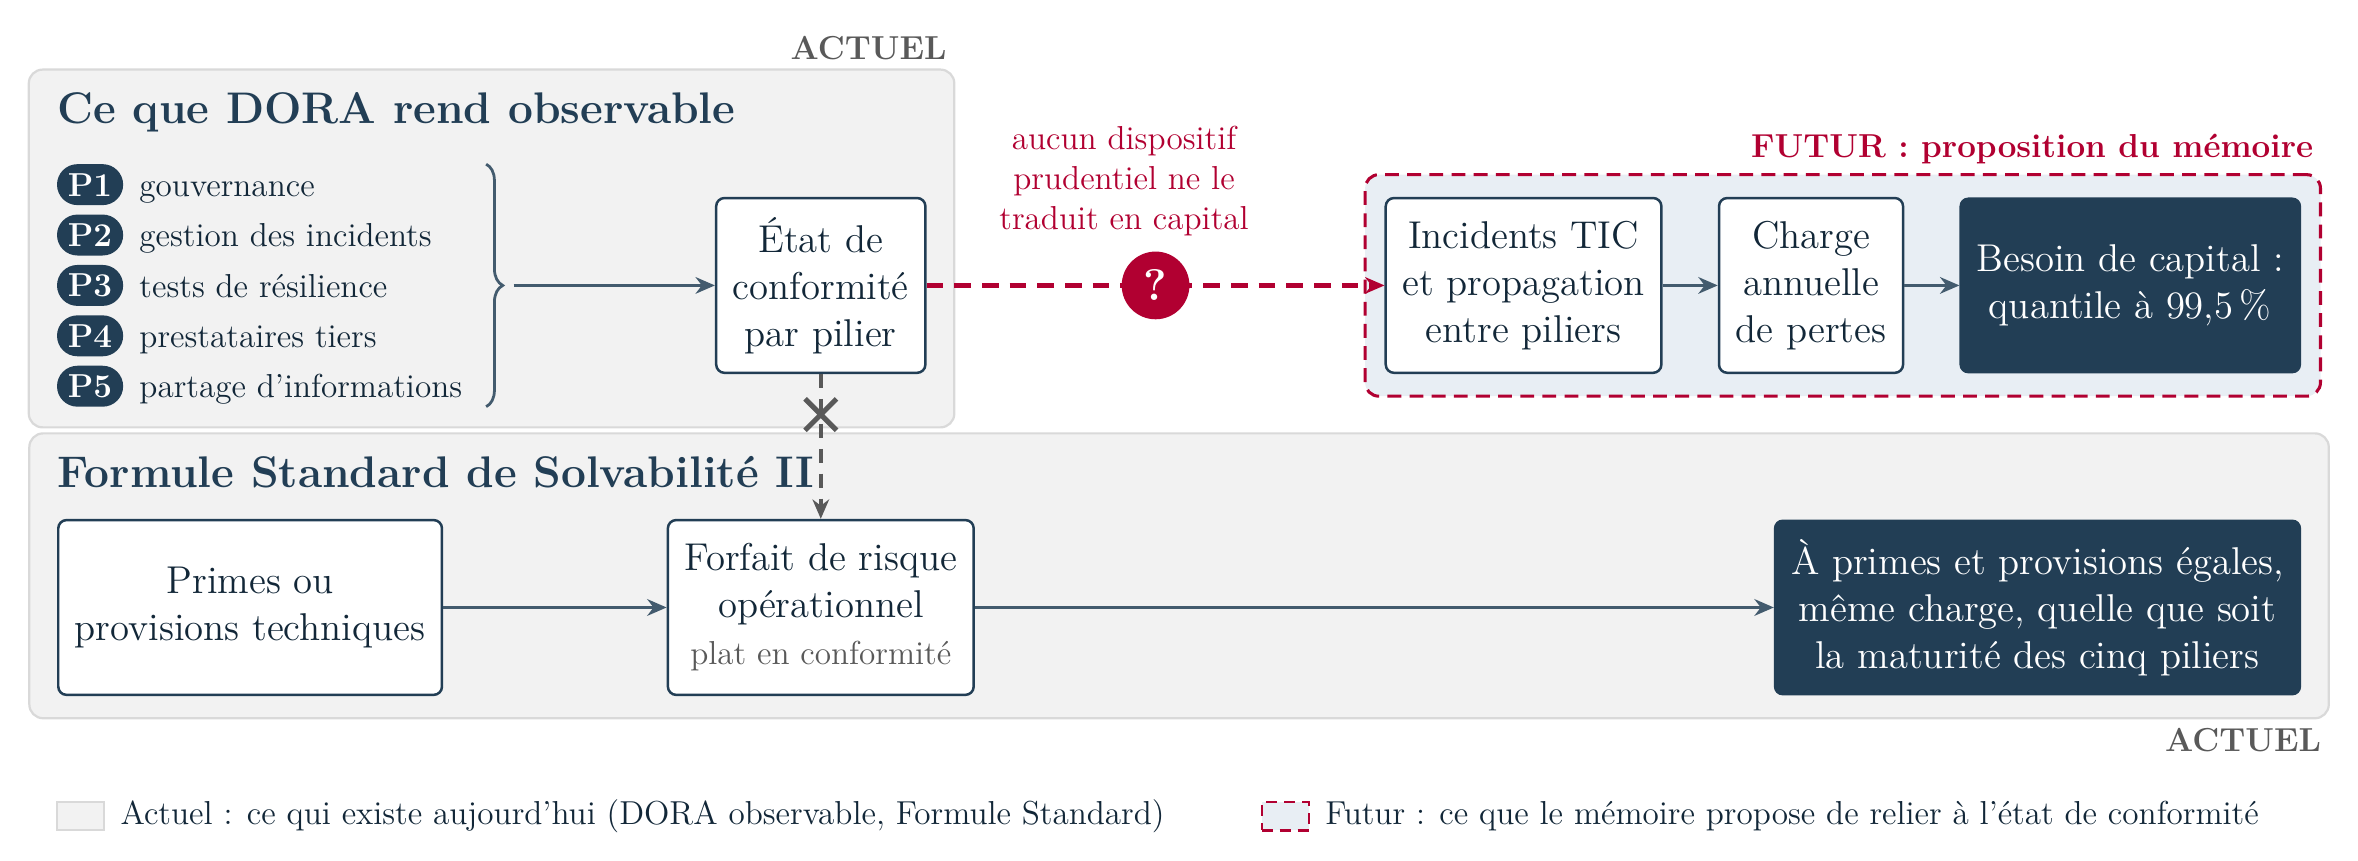
\begin{tikzpicture}[x=1cm,y=1cm]
  \def\yT{-2.46}   % axe de la voie du haut (centre de la colonne des piliers)
  \def\yB{-6.55}   % axe de la voie du bas
  \def\xC{9.7}     % abscisse commune de l'etat de conformite et du forfait

  % ---------------- voie du haut ----------------
  \node[anchor=north west, inner sep=0, font=\grand\bfseries, text=ardoise]
    (titreh) at (0,0) {Ce que DORA rend observable};

  \foreach \i/\lab in {1/gouvernance, 2/gestion des incidents, 3/tests de résilience,
                       4/prestataires tiers, 5/partage d’informations} {
    \pgfmathsetmacro{\y}{-1.18-0.64*(\i-1)}
    \node[rounded corners=0.26cm, fill=ardoise, text=white, font=\petit\bfseries,
          inner sep=0, minimum width=0.84cm, minimum height=0.52cm] (p\i) at (0.42,\y) {P\i};
    % meme ligne de base que « P\i », dont la boite n'a pas de jambage
    \node[anchor=base west, inner sep=0, font=\petit, text=encre] (l\i) at (1.04,\y-0.148) {\lab};
  }
  \draw[decorate, decoration={brace, amplitude=6pt}, line width=1pt, draw=acier]
    (5.45,-0.92) -- (5.45,-4.0);

  \node[bloc, minimum height=2.22cm] (conf) at (\xC,\yT)
    {État de\\conformité\\par pilier};
  \draw[fleche] (5.8,\yT) -- (conf.west);

  \node[bloc plein, font=\corps, minimum height=2.22cm, anchor=east] (cap)
    at (28.5,\yT) {Besoin de capital~:\\quantile à 99,5\,\%};
  \node[bloc, minimum height=2.22cm, left=0.7cm of cap] (charge)
    {Charge\\annuelle\\de pertes};
  \node[bloc, minimum height=2.22cm, left=0.7cm of charge] (inc)
    {Incidents TIC\\et propagation\\entre piliers};
  \draw[fleche] (inc) -- (charge);
  \draw[fleche] (charge) -- (cap);

  % maillon manquant : le seul element en accent
  \draw[fleche accent, dash pattern=on 6pt off 4pt] (conf.east) -- (inc.west);
  \coordinate (m) at ($(conf.east)!0.5!(inc.west)$);
  \node[circle, fill=accent, text=white, font=\grand\bfseries, inner sep=0,
        minimum size=0.86cm] at (m) {?};
  \node[anchor=south, font=\petit, text=accent, align=center, inner sep=0]
    at ($(m)+(-0.4,0.62)$) {aucun dispositif\\prudentiel ne le\\traduit en capital};

  % ---------------- voie du bas ----------------
  \node[anchor=north west, inner sep=0, font=\grand\bfseries, text=ardoise]
    (titreb) at (0,-4.62) {Formule Standard de Solvabilité II};

  \node[bloc, minimum height=2.22cm, anchor=west] (prim)
    at (0,\yB) {Primes ou\\provisions techniques};
  \node[bloc, minimum height=2.22cm] (forf) at (\xC,\yB)
    {Forfait de risque\\opérationnel\\{\petit\color{gris}plat en conformité}};
  \node[bloc plein, font=\corps, minimum height=2.22cm, anchor=east] (meme)
    at (28.5,\yB) {À primes et provisions égales,\\même charge, quelle que soit\\la maturité des cinq piliers};
  \draw[fleche] (prim) -- (forf);
  \draw[fleche] (forf) -- (meme);

  % lien barre : la voie du bas ne recoit rien de l'etat de conformite
  \draw[fleche, draw=gris, dash pattern=on 5pt off 4pt] (conf.south) -- (forf.north);
  \coordinate (x) at (\xC,-4.1);
  \draw[gris, line width=1.8pt] ($(x)+(-0.2,-0.2)$) -- ($(x)+(0.2,0.2)$)
                                ($(x)+(-0.2,0.2)$) -- ($(x)+(0.2,-0.2)$);

  % ---------------- fonds : actuel (gris) et futur (bleu, liseré rouge) ----------------
  \begin{scope}[on background layer]
    % actuel, voie du haut : les cinq piliers et leur etat de conformite
    \node[fit=(titreh)(p1)(l5)(conf), fill=clair, draw=filet, line width=0.8pt, rounded corners=5pt,
          inner xsep=10pt, inner ysep=8pt] (act1) {};
    % actuel, voie du bas : la Formule Standard
    \node[fit=(titreb)(prim)(meme), fill=clair, draw=filet, line width=0.8pt, rounded corners=5pt,
          inner xsep=10pt, inner ysep=8pt] (act2) {};
    % futur : la chaine des pertes que le memoire relie a l'etat de conformite
    \node[fit=(inc)(charge)(cap), fill=futur, draw=accent, line width=1.1pt, dash pattern=on 5pt off 3pt,
          rounded corners=5pt, inner xsep=7pt, inner ysep=8pt] (fut) {};
  \end{scope}
  \node[anchor=south east, font=\petit\bfseries, text=gris, inner sep=3pt] at (act1.north east) {ACTUEL};
  \node[anchor=north east, font=\petit\bfseries, text=gris, inner sep=3pt] at (act2.south east) {ACTUEL};
  \node[anchor=south east, font=\petit\bfseries, text=accent, inner sep=3pt] at (fut.north east) {FUTUR : proposition du mémoire};

  % ---------------- legende ----------------
  \def\yL{-9.2}
  \node[draw=filet, fill=clair, line width=0.8pt, minimum width=0.6cm, minimum height=0.36cm] (k1) at (0.3,\yL) {};
  \node[anchor=west, font=\petit, text=encre, inner sep=0] at (0.8,\yL)
    {Actuel : ce qui existe aujourd’hui (DORA observable, Formule Standard)};
  \node[draw=accent, fill=futur, line width=0.9pt, dash pattern=on 4pt off 2.5pt, minimum width=0.6cm,
        minimum height=0.36cm] (k2) at (15.6,\yL) {};
  \node[anchor=west, font=\petit, text=encre, inner sep=0] at (16.1,\yL)
    {Futur : ce que le mémoire propose de relier à l’état de conformité};
\end{tikzpicture}
\end{document}
